\documentclass[tikz,convert={outext=.svg,command=\unexpanded{pdf2svg \infile\space\outfile}},multi=false]{standalone}
\usepackage[utf8]{inputenc}

\usetikzlibrary{automata}% tikz package already loaded by 'tikz' option
\newcommand{\ascenseur}[5]{\begin{tikzpicture}[xscale=0.7]
\draw[draw=#5] (-0.3, 1.1) -- (-0.3, 1.5);
\draw[draw=#5] (-0, 1.1) -- (-0, 1.5);
\draw[draw=#5] (0.3, 1.1) -- (0.3, 1.5);
\draw[draw=#5] (-0.3, 0.9) -- (-0.3, 0.5);
\draw[draw=#5] (-0, 0.9) -- (-0, 0.5);
\draw[draw=#5] (0.3,0.9) -- (0.3,0.5);
\draw (-1, 2) -- (-1, 0) -- (1, 0) --(1, 2);
\draw[fill=#1, draw=none] (-0.8, 1) rectangle (0.8, 0);
\draw[fill=#2, draw=none] (-0.8, 2) rectangle (0.8, 1);
\draw[fill=#3] (1, 0.4) rectangle (1.2, 0.6);
\draw[fill=#4] (1, 1.4) rectangle (1.2, 1.6);
\end{tikzpicture}}
\begin{document}


\newcommand\xm5
\newcommand\xM{10}
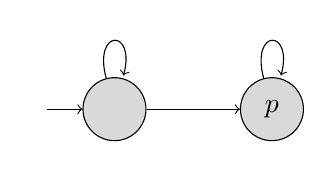
\begin{tikzpicture}
\tikzstyle{etat} = [draw, circle, fill=gray!30, minimum height=8mm];
%\node (0bbm) {\ascenseur {black} {none} {white} {white} {white}};
%\node (0Bbm) at (\xm, 2) {\ascenseur {black} {none} {black} {white} {white}};
%\node (0BbM) at (\xM, 2) {\ascenseur {black} {none} {black} {white} {black}};
%\node (0bBm) at (\xm, -2) {\ascenseur  {black} {none}  {white} {black} {white}};
%\node (0bBM) at (\xM, -2) {\ascenseur {black} {none}  {white} {black} {black}};
%
%\node (0BBm) at (\xm, 0) {\ascenseur  {black} {none}  {black} {black} {white}};
%\node (0BBM) at (\xM, 0) {\ascenseur {black} {none}  {black} {black} {black}};
%
%\node (1bbm) at (0, 8) {\ascenseur {none} {black} {white} {white} {white}};
%\node (1Bbm) at (\xm, 10) {\ascenseur {none} {black} {black} {white} {white}};
%\node (1BbM) at (\xM, 10) {\ascenseur {none} {black} {black} {white} {black}};
%\node (1bBm) at (\xm, 6) {\ascenseur  {none} {black}  {white} {black} {white}};
%\node (1bBM) at (\xM, 6) {\ascenseur {none} {black}  {white} {black} {black}};
%
%\node (1BBm) at (\xm, 8) {\ascenseur   {none} {black}  {black} {black} {white}};
%\node (1BBM) at (\xM, 8) {\ascenseur  {none} {black}  {black} {black} {black}};
%
%\draw[->] (0bbm) edge (0Bbm);
%\draw[->] (0bbm) edge (0bBm);
%\draw[->] (0Bbm) edge (0BBm);
%\draw[->] (0bBm) edge (0BBm);
%
%\draw[->] (0bBm) edge (0bBM);
%\draw[->] (0bBm) edge (0bBM);
%\draw[->] (0BBm) edge (0BBM);
%
%\draw[->] (1bbm) edge (1Bbm);
%\draw[->] (1bbm) edge (1bBm);
%\draw[->] (1Bbm) edge (1BBm);
%\draw[->] (1bBm) edge (1BBm);
%
%\draw[->] (1Bbm) edge (1BbM);
%
%\draw[->] (0bBM) edge [bend right=10] (1bbm);
%\draw[->] (1BbM) edge [bend right=-10] (0bbm);
%\draw[->] (0BBM) edge  (1bBm);

\node[etat, initial left, initial text={}] (a) {};
\node[etat] (s)  at (2, 0) {$p$};
\draw[->] (a) edge[loop above] (a);
\draw[->] (s) edge[loop above] (s);
\draw[->] (a) -- (s);
\end{tikzpicture}
\end{document}